%!TEX root = ../../thesis.tex
\section{Digest Loop and Scopes}

Scopes have already been mentioned in the last chapter, but they were only introduced briefly. They are an essential part of AngularJS's inner event cycle which is called the `digest cycle'. When an AngularJS application is initialized, a \code{rootScope} is created which is a scope that can be accessed by any component and from which all child scopes are created from. Each controller instance in an application gets its own \code{scope} instance which is inherited prototypically from the parent scope. The first controllers that are created will get a \code{scope} that inherits from the \code{rootScope} and all controllers that are created as child controllers will inherit from their parent's controller. So each \code{scope} indirectly inherits from the \code{rootScope}.

\begin{figure}[htb]
  \centerline{
    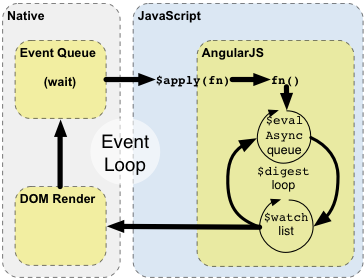
\includegraphics[width=0.8\linewidth]{images/concepts-runtime.png}
  }
  \caption[digest cycle (source: \url{https://docs.angularjs.org/guide/scope})]{digest cycle (source: \url{https://docs.angularjs.org/guide/scope})}
  \label{fig:digest-loop}
\end{figure}

As mentioned before, scopes are important for AngularJS's digest loop which is the core component that enables data binding and expression watching. The cycle is demonstrated in \reffigure{fig:digest-loop}. It shows that AngularJS's digest loop is triggered by the browser's event loop. If for example a click event is detected, the digest loop is initialized by applying the event's callback in AngularJS's digest loop. This will then initialize a loop over all watchers which will execute all \code{\$watch} listeners that are either created manually in controllers or internally by template bindings. This loop is executed until there are no more changes happening in the watcher functions. This needs to be done, because watchers are actually allowed to change the state of the application and by that they can trigger other watcher functions. Obviously, this loop has a limited number of runs, because watchers might create infinite loops by altering state that is watched by others, who then alter state that they were originally watching. After the loop has finished executing all watchers, the current scope's template and all other templates that have changed values are updated.

AngularJS's digest loop is often a concept that is hard to understand when starting to work with it, because it leads to problems when working with external libraries. If for example an asynchronous library is used and the scope is changed in a callback that is passed into this library, the changes will not trigger any of the watchers. This is due to AngularJS not knowing about the callback and not knowing about the changes that were done in this callback. In these cases, the callback needs to be wrapped into a scope's \code{\$apply(fn)} function which will trigger the digest loop manually.